\documentclass[10pt,twocolumn,letterpaper]{article}
\usepackage[review]{cvpr}
\usepackage{array}
\usepackage{microtype}
\definecolor{cvprblue}{rgb}{0.21,0.49,0.74}
\usepackage[pagebackref,breaklinks,colorlinks,allcolors=cvprblue]{hyperref}
\usepackage[capitalize]{cleveref}
\def\confName{CVPR}
\def\confYear{2027}
\title{Beyond Spread: Diagnosing and Repairing Gaps in Generative Distributions}
\author{}
\hypersetup{pdftitle={Beyond Spread: Diagnosing and Repairing Gaps in Generative Distributions},pdfauthor={}}
\raggedbottom
\setlength{\hfuzz}{0.5pt}
\begin{document}
\maketitle
\begin{abstract}
Two image generators can produce equally varied images while one of them
has lost an entire part of the image distribution. We introduce an audit
that compares a generator with a fixed set of reference images. It
measures how much probability each part of the image space gains or
loses, how varied the images within each part are, and whether a
targeted change improves the intended outcome on fresh images. The audit
also states in advance how large a loss must be to count and how many
images are needed to detect it. On CIFAR-10 with a two-step sampler,
changing only the covariance of the starting noise lowers the distance
to real images by 32\%. On MNIST, ordinary training corrects a digit that
targeted training had overshot, reducing the mean error in digit
frequencies by 59\% at the same training budget. In text-to-image
generation, the audit explains how variation pooled across prompts can
fall while variation within each prompt rises.
\end{abstract}

\begin{figure*}[t]
\centering
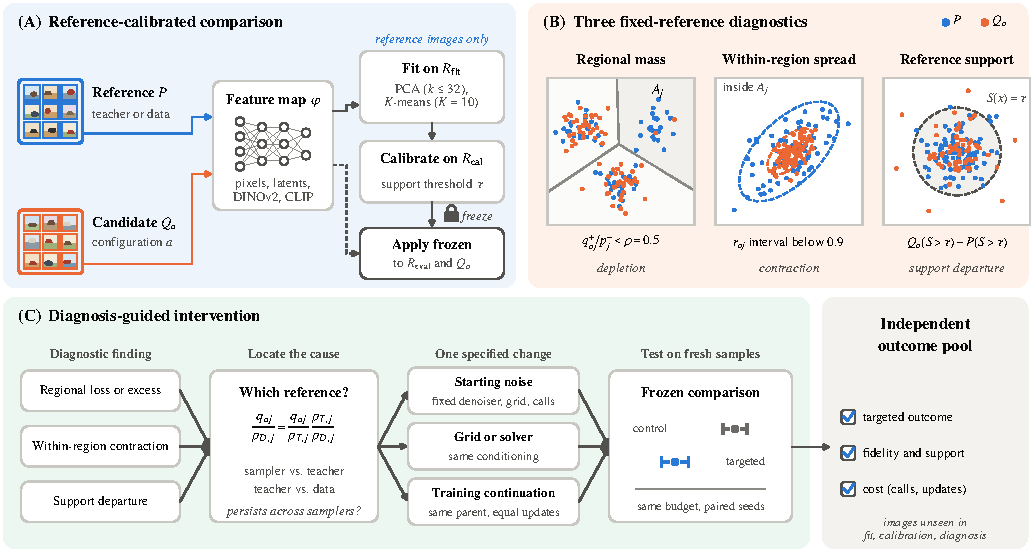
\includegraphics[width=\textwidth,pagebox=cropbox]{../figures/pipeline_overview.pdf}
\caption{Fixed-reference diagnosis and repair. (A) Reference and candidate
images share the feature map $\phi$; regions are fit on $R_{\rm fit}$, the
support threshold is calibrated on $R_{\rm cal}$, and both are frozen before
evaluation. (B) Three diagnostics: regional mass, within-region spread, and
reference support. (C) A diagnosis motivates one specified change, tested
against its control on independent outcomes. Images and point clouds are
illustrative.}
\label{fig:pipeline}
\end{figure*}

\section{Introduction}
\label{sec:intro}
Two generators can have the same global variance while assigning very
different probabilities to parts of the image distribution. For a
few-step sampler, that difference determines what needs to change.
Changing the starting noise can recover image neighborhoods lost during
sampling. A digit that remains absent under several adequate samplers
calls for a test of the training distribution. The two cases require
different controls and different outcomes.

Existing occupancy tests can detect a change in a fixed region
\cite{richardson2018ndb}. To act on that change, however, we need to know
how large it is, what reference it is relative to, and whether an
intervention improves the target without violating fidelity criteria.
An equality test does not answer these questions, and a pooled measure
of spread can stay unchanged while a region is lost.

We therefore fix the reference, the regions, and the effect sizes before
evaluation (Fig.~\ref{fig:pipeline}). A longer teacher sampler measures
the change introduced by a faster sampler, and observed data can reveal an
imbalance shared by both. Conditional spread then measures variation among
samples in the same region or under the same prompt, separately from
regional probability. Each diagnosis motivates one specified change, which
is tested against its control on fresh samples. We ask three questions.
Which regions lose or gain probability relative to a fixed reference?
How does variation within a region or prompt change when fidelity is
measured separately? Which controlled interventions repair the diagnosed
deficit on independent samples?

Two confirmed repairs demonstrate this approach (Fig.~\ref{fig:overview}).
On CIFAR-10, covariance initialization reduces two-call Kernel Inception
Distance (KID) by 32.0\% and increases real-data DINO coverage from 0.206
to 0.288. Evaluating the same outputs against a separate CIFAR-10.1 reference
gives 32.7\% lower KID. On MNIST, signed regional measurements identify
overcorrection after targeted restoration. A separate equal-update
ordinary-data continuation lowers class-mass error by 58.7\% within the
declared fidelity margins.

\begin{figure}[t]
\centering
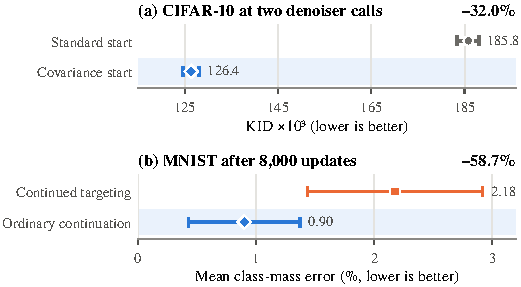
\includegraphics[width=\linewidth]{../figures/overview.pdf}
\caption{Two matched-budget repairs. (a) Covariance start versus standard
start at two denoiser calls on CIFAR-10. (b) Ordinary continuation versus
continued targeting after 8,000 MNIST updates. Bars are 95\% intervals
(Sec.~\ref{sec:metrics}).}
\label{fig:overview}
\end{figure}

A toy example shows why spread alone is not enough. Consider a reference
with probabilities $(1/4,1/2,1/4)$ at feature values $(-2,0,2)$ and a
candidate with equal mass at $-\sqrt{2}$ and $\sqrt{2}$. Both have mean
zero and variance two. The fixed region $[-1/2,1/2]$ contains half the
reference mass and zero candidate mass. If 100 independent draws per
distribution give 50 reference hits and zero candidate hits, the
one-region audit gives a 97.5\% simultaneous upper bound of 0.133 on the
mass ratio. This certifies depletion at the declared threshold of 0.5
(Sec.~\ref{sec:mass}).

Our paper offers the following contributions. First, we introduce a
fixed-reference audit that distinguishes regional loss, within-region
contraction, and departures from reference support, and whose
finite-sample bounds show how the resolution of a regional diagnosis
depends on the effect size, the reference mass, and the comparison family.
Second, we use these diagnoses to design two matched-budget repairs,
a covariance-matched starting noise for a few-step sampler and an
ordinary-data continuation after targeted training, and confirm both on
independent samples. Third, we explain why pooled spread, within-prompt
spread, and comparisons to different teachers can give different answers
about the same generator, using text-to-image models as the test case.

Section~\ref{sec:related} reviews related work, and Sec.~\ref{sec:method}
defines the audit and its guarantees. Section~\ref{sec:experiments}
describes the data, settings, baselines, and metrics.
Section~\ref{sec:results} reports the repairs, the controls, and the
resolution of the audit, and Sec.~\ref{sec:conclusion} concludes.

\section{Related work}
\label{sec:related}
Global fidelity and coverage metrics~\cite{kynkaanniemi2019improved,naeem2020density,alaa2022faithful}
and kernel diversity scores~\cite{friedman2023vendi,ospanov2025scendi}
summarize a whole distribution or its prompt-conditioned variation, and
Conditional Vendi and R\'enyi kernel entropy also use the prompt/model
decomposition to guide generation~\cite{jalali2026conditional}. The
closest regional analysis is the NDB test, which compares occupancy in
fixed $K$-means regions~\cite{richardson2018ndb}. Our audit inherits its
fixed regions but replaces the equality test with an effect-size
certificate, whose resolution Corollary~1 states in advance, and adds
conditional spread and a calibrated support gate so that each finding
maps to a testable intervention.

Few-step interventions can change the solver, the generator, or the
conditions at sampling time. DDIM, DPM-Solver++, and UniPC change how a
fixed denoiser is integrated~\cite{song2021ddim,lu2022dpmpp,zhao2023unipc},
while consistency and distribution-matching distillation change the
learned generator~\cite{luo2024lcm,luo2023lcmlora,yin2024dmd2}.
Data-dependent priors, starting-noise corrections, and schedule design
address the match between initial noise and the sampler
\cite{lee2022priorgrad,zheng2023truncated,hu2024onemore,lin2024flawed,sabour2024align}.
Conditioning noise, early-step hybrids, covariance-aware sampling, and
adaptive computation provide other intervention points
\cite{sadat2024cads,gandikota2026diversity,schioppa2026covariance,zhang2025adadiff,li2024budgetfusion,binici2026adsc}.
Exact Gaussian solutions and spectral transfer analyses distinguish
initialization from integration error~\cite{pierret2025gaussian,benita2025spectral}.
We use this distinction to test a covariance-only change on a fixed
denoiser and time grid, and account separately for the cost of diagnosing
a deficit and generating new images.

\section{A fixed-reference audit for distribution repair}
\label{sec:method}
The audit fixes a reference and regional targets, measures mass, spread,
and support, and tests a diagnosis-guided intervention on independent
outcomes (Fig.~\ref{fig:pipeline}; Supp.~Algorithm~1).

\subsection{Setting and notation}
\label{sec:setting}
Let $\mathcal X$ be the image space. A configuration $a$ specifies the
checkpoint, schedule, guidance, solver, and randomization of a generator,
and $Q_a$ denotes its output law on $\mathcal X$. The audit compares $Q_a$
with a reference law $P$. We use the law $P_T$ of a resolved teacher to
measure sampler-relative change, or the observed-data law $P_D$ to measure
data-relative representation. Before evaluation we declare the
representation, regions, effect sizes, fidelity margins, comparison
family, and budget.

Disjoint reference pools fit the regions and support score
($R_{\rm fit}$), calibrate the threshold ($R_{\rm cal}$), and estimate
reference outcomes ($R_{\rm eval}$). Candidate images enter neither
fitting nor calibration. A diagnosis pool selects the intervention;
an independent outcome pool evaluates the frozen comparison. The audit
reports regional decisions and intervals, conditional spread, fidelity,
and cost.

\subsection{Representation, regions, and pooled spread}
\label{sec:regions}
A representation $\phi:\mathcal X\to\mathbb R^d$ maps an image to $d$
features. Pixel, latent, DINOv2, and CLIP features offer different views
of the images~\cite{oquab2024dinov2,radford2021clip}. Principal component
analysis (PCA) fitted on $R_{\rm fit}$ gives a mean $m\in\mathbb R^d$,
an orthonormal basis $U\in\mathbb R^{d\times k}$ of $k$ retained
directions, and coordinates $z(x)=U^\top(\phi(x)-m)\in\mathbb R^k$.
For feature regions, we scale each coordinate of $z$ by its reference-fit
standard deviation and fit $K$ $K$-means cells to the scaled coordinates.
The regions use these scaled coordinates, the spread ratio of
\cref{eq:spread} uses $z$ itself, and the support score of
\cref{eq:support} uses whitened coordinates. The fixed assignment
$J(x)\in\{1,\ldots,K\}$ defines the regions $A_j=\{x:J(x)=j\}$, which
partition $\mathcal X$.

For semantic regions, the same classifier and rejection rule are applied
to both laws. The partition includes rejection, so rejected images stay
in the denominator of each region's probability. Held-out real accuracy
validates the labeling rule on real images. Feature fidelity and
uncurated samples help assess its interpretation on generated images.

Write the regional masses as $p_j=P(X\in A_j)$ and
$q_{aj}=Q_a(X\in A_j)$. Under $P$, let $Y=\phi(X)$ have mean $\mu$,
with conditional mean $\mu_j$ and covariance $\Sigma_j$ in $A_j$.
The law of total covariance gives
\begin{equation}
\operatorname{Cov}_{P}(Y)
=\sum_j p_j\Sigma_j+\sum_j p_j(\mu_j-\mu)(\mu_j-\mu)^\top,
\label{eq:totalcov}
\end{equation}
with zero-mass terms contributing zero. Pooled spread combines
within-region variation, regional separation, and their probability
weights; the audit measures mass and conditional spread separately.

\subsection{Certifying a regional change in mass}
\label{sec:mass}
To certify a regional change, we fix all events before drawing evaluation
images independently within each law. Reference and candidate draws may
be paired across laws. The guarantee assumes fixed evaluation sizes.
Pooling samples drawn under different prompts requires a sampling model
for the prompt mixture, so we report prompt-level uncertainty separately.

Let $M$ count all declared region, condition, configuration, and
representation comparisons, and let $\alpha_{\rm occ}$ be the family
error budget. Let $[p_j^-,p_j^+]$ and $[q_{aj}^-,q_{aj}^+]$ be exact
binomial intervals~\cite{clopper1934confidence} with per-tail error
$\varepsilon=\alpha_{\rm occ}/(4M)$.

\paragraph{Proposition 1 (simultaneous ratio intervals).}
\emph{With probability at least $1-\alpha_{\rm occ}$, every positive-mass
region in the family satisfies}
\begin{equation}
q_{aj}/p_j\in\left[q_{aj}^-/p_j^+,\ q_{aj}^+/p_j^-\right].
\label{eq:occupancy}
\end{equation}

\noindent\emph{Proof.} A union bound over the $4M$ one-sided endpoints
gives simultaneous coverage at least $1-\alpha_{\rm occ}$; monotonicity of the
ratio gives \cref{eq:occupancy}. \hfill$\square$

For $p_j>0$, the upper endpoint is infinite when $p_j^-=0$. Only eligible
regions receive a ratio decision. An eligible region has
$p_j^-\geq\pi_{\min}$, a minimum reference mass. An upper endpoint below
the ratio threshold $\rho$ certifies \emph{depletion}; a lower endpoint
above $\rho$ certifies \emph{retention} at that resolution. Otherwise the
test is unresolved. For signed mass balance, we bound $q_{aj}-p_j$ by
$[q_{aj}^--p_j^+,q_{aj}^+-p_j^-]$ with a margin $\delta>0$. The interval
must lie below, above, or within $[-\delta,\delta]$ to certify depletion,
excess, or equivalence, respectively.

\paragraph{Corollary 1 (samples needed).}
\emph{Suppose a region is eligible, $0<\rho p_j^-<1$, and none of $n_Q$
candidate draws falls in it. Then \cref{eq:occupancy} certifies depletion
if and only if}
\begin{equation}
n_Q>\frac{\log\varepsilon}{\log(1-\rho p_j^-)}.
\label{eq:planning}
\end{equation}

\noindent\emph{Proof.} With zero candidate hits,
$q_{aj}^+=1-\varepsilon^{1/n_Q}$; solving
$q_{aj}^+<\rho p_j^-$ gives \cref{eq:planning}. \hfill$\square$

The bound makes the sample cost of rare regions and broad comparison
families explicit.

\subsection{Conditional spread}
\label{sec:spread}
To measure variation separately from mass, we compare the covariance
traces of the unwhitened coordinates within $A_j$:
\begin{equation}
r_{aj}=\frac{\operatorname{tr}\operatorname{Cov}_{Q_a}[z(X)\mid A_j]}
{\operatorname{tr}\operatorname{Cov}_{P}[z(X)\mid A_j]}.
\label{eq:spread}
\end{equation}
This ratio is defined when the region has positive mass under both laws
and the reference trace is positive. The trace sums coordinate variances
after centering each law separately. Approximate influence-function
intervals for $\log r_{aj}$ lying wholly below or above declared margins
flag contraction or expansion. For text-to-image generation, we divide
the mean within-prompt trace of the candidate by that of the reference
in each representation and bootstrap whole matched prompts.

\subsection{Reference support}
\label{sec:support}
A support score $S(x)$ combines the whitened distance to the nearest
reference-fit point and the scaled PCA residual norm in quadrature:
\begin{equation}
S(x)=\sqrt{d_{\rm NN}(x)^2+
\bigl(\|\phi(x)-m-Uz(x)\|_2/s_{\rm res}\bigr)^2},
\label{eq:support}
\end{equation}
where $d_{\rm NN}(x)$ is the nearest fit-sample distance in whitened PCA
coordinates and $s_{\rm res}$ is the residual scale (Supp.~Sec.~C.1).
The residual captures departures in directions discarded by projection.
With $n_{\rm cal}$ exchangeable reference calibration samples, the
threshold $\tau$ is the $\lceil(n_{\rm cal}+1)0.95\rceil$-th score in
ascending order~\cite{vovk2013conditional}. If this rank is unavailable,
the gate is unresolved. Independent evaluations estimate the excess tail
probability $Q_a(S>\tau)-P(S>\tau)$, which exact binomial endpoints bound
(Supp.~Sec.~A.3). The gate passes if the upper bound is at most a declared
tolerance and fails if the lower bound exceeds it. Otherwise it is
unresolved. Expansion with a failed support gate is off-reference expansion.

\subsection{From diagnosis to a controlled intervention}
\label{sec:intervene}
For the same semantic event, let $p_{D,j}=P_D(A_j)$ and $p_{T,j}=P_T(A_j)$.
When both are positive,
\begin{equation}
\frac{q_{aj}}{p_{D,j}}=\frac{q_{aj}}{p_{T,j}}\cdot\frac{p_{T,j}}{p_{D,j}}
\label{eq:decomp}
\end{equation}
separates sampler--teacher from teacher--data mass differences.
Teacher-relative deficits motivate a starting-noise change at fixed
denoiser, grid, and call budget, or a solver/grid comparison under the
same conditioning. A validated data-relative imbalance persisting across
qualified samplers motivates ordinary versus targeted continuation from
the same parent at equal update budgets. After diagnosis, we freeze one
change and its control, then evaluate the targeted outcome, fidelity,
coverage, and cost on independent samples.

\paragraph{Why the starting covariance matters.}
Common schedules with leading timestep spacing start sampling from a
noise level that the standard Gaussian does not match~\cite{lin2024flawed},
and data-dependent priors change the starting distribution through
training~\cite{lee2022priorgrad}. We quantify the effect of the mismatch
and test a training-free correction. Consider a centered clean Gaussian
coordinate $X_0$ with variance
$\lambda>0$. Variance-preserving noising gives
$X_t=\sqrt{\bar\alpha_t}X_0+\sqrt{1-\bar\alpha_t}\,\epsilon$ at
timestep $t$, with cumulative signal coefficient $\bar\alpha_t\in[0,1]$
and independent $\epsilon\sim\mathcal N(0,1)$. Write
$v_t=\bar\alpha_t\lambda+1-\bar\alpha_t$ for the noisy variance and
$u_t=(\sqrt{\bar\alpha_t\lambda},\sqrt{1-\bar\alpha_t})$.
Let $X_{\rm out}$ be the final coordinate, and let $\nu_{\rm start}$ and
$v_{\rm start}$ be the actual and matched starting variances.

\paragraph{Proposition 2 (initialization and integration).}
\emph{With the conditional mean noise predictor
$\mathbb E[\epsilon\mid X_t]$ and no clipping, a deterministic DDIM
transition to an earlier timestep $s$ multiplies the coordinate by
$\sqrt{v_s/v_t}\cos\angle(u_s,u_t)$. On a fixed grid, the variance factors
telescope to the clean endpoint:}
\begin{equation}
\frac{\operatorname{Var}(X_{\rm out})}{\lambda}
=\underbrace{\frac{\nu_{\rm start}}{v_{\rm start}}}_{\text{initialization}}
\underbrace{\prod_{t\rightarrow s}\cos^2\angle(u_s,u_t)}_{\text{integration}},
\label{eq:gaussian}
\end{equation}
\emph{where the product runs over adjacent grid transitions.}

The derivation builds on exact Gaussian analyses
\cite{benita2025spectral,pierret2025gaussian}
(Supp.~Secs.~D--F). Matching the noisy marginal sets the initialization
factor to one; refining a grid with fixed endpoints improves the
integration factor. Changing the leading-grid budget also changes the
starting timestep. \Cref{eq:gaussian} extends directionwise to shared
eigenvectors.

For a leading grid starting at timestep $t_0$, the tested initializer is
\begin{equation}
X_{\rm start}=
\big[(1-\bar\alpha_{t_0})I+\bar\alpha_{t_0}\widehat C\big]^{1/2}Z,
\qquad Z\sim\mathcal N(0,I),
\label{eq:covariance_start}
\end{equation}
where $X_{\rm start}$ is the initial noisy image, $Z$ is standard Gaussian
noise, $I$ is the identity in pixel space, $\widehat C$ is an estimate of
the clean covariance, and the square root is symmetric. We call this the
\emph{covariance start} and the usual $X_{\rm start}=Z$ the
\emph{standard start}. The covariance start adds no denoiser calls.

\subsection{Implementation details}
\label{sec:implementation}
We retain up to $k=32$ PCA directions and fit $K=10$ $K$-means cells.
Depletion uses $\rho=0.5$ and $\pi_{\min}=0.01$ by default, and the digit
study uses $\delta=0.03$ and charges the shared reference bounds once
(Supp.~Sec.~C.8). A finite estimated log-ratio spread interval requires at
least 30 samples from each law and positive sample trace in both;
intervals wholly below 0.9 or above 1.1 flag contraction or expansion.
The residual scale $s_{\rm res}$ is the median fit residual, floored at
$10^{-6}$, and the support gate tolerance is 0.05. The feature-only
default gives occupancy and support error budgets of 0.025 each. The
approximate spread intervals are outside that exact error guarantee.
Signed-balance and routing follow-ups allocate 0.025/0.0125/0.0125 to
mass/fidelity/support. CIFAR selection also checks teacher precision,
text-to-image checks alignment and learned preference, and digits use
classifier consensus and feature precision. For CIFAR-10, $I$ is the
identity in 3,072-dimensional pixel space, $\widehat C$ uses 128
teacher-fit pixel components and an isotropic residual, and the two-call
grid starts at $t_0=500$.

\section{Experiments}
\label{sec:experiments}
An \emph{arm} is a generator configuration; a \emph{panel} is an
independently generated sample set. A \emph{resolved probe} is a longer
sampler that passes its fidelity gates. Gates compare intervals with
declared margins and return pass, fail, or unresolved. Comparisons are
\emph{frozen} before outcome sampling.

\subsection{Datasets}
\label{sec:datasets}
We validate the audit's resolution on controlled deletions from Gaussian
mixtures and from cached image features, where the removed region and
its mass are known. The image experiments use four settings.
CIFAR-10 uses a public pretrained DDPM~\cite{krizhevsky2009cifar,ho2020ddpm}.
A 20,000-image DDIM100 teacher supplies 5,000/5,000/10,000 disjoint
fitting/calibration/evaluation images. CIFAR-10.1v6~\cite{recht2018cifar10}
provides a second, separately collected real reference of 2,000 images,
and an independently pretrained variance-preserving EDM
model~\cite{karras2022edm} provides a second checkpoint for solver
comparisons. For CIFAR-10 semantic regions, classifier consensus defines ten
accepted classes plus rejection; real-image consensus acceptance is
90.75\%, with 98.75\% accuracy among accepted images.

In MNIST~\cite{lecun1998mnist}, withholding digit~3 from training creates
a known data-relative deficit. Two calibrated classifiers define consensus
digit regions and rejection; accepted real-image accuracy is 99.916\%, and
rejection remains in every probability denominator. For text-to-image
generation, we compare SD1.5, native LCM-LoRA, one-step DMD2, and Sana-600M
\cite{rombach2022ldm,luo2023lcmlora,yin2024dmd2,xie2025sana} on 128 held-out
PartiPrompts~\cite{yu2022parti}. Disjoint pools supply 32 representation-fit,
256 calibration, and 48 development prompts. References are DDIM50 at
classifier-free guidance (CFG) 7.5 and Flow-DPM++50; DMD2 also uses its
training-matched CFG1.75 teacher. These are generator-relative
measurements; prompts supply no real-image coverage target.

\subsection{Experimental settings}
\label{sec:settings}
Leading timestep spacing starts the two-call CIFAR-10 grid at $t_0=500$;
trailing spacing starts at the final timestep. We evaluate 22 sampler
and initialization arms at two, four, and eight calls, using a
2,048-image pilot and 10,000 fresh images per arm. A separate six-arm
confirmation uses five fresh paired panels of 2,000 images
(Fig.~\ref{fig:cifar_initializer}a). At four and eight calls, matched-grid
controls share trailing timesteps. Covariance-aware sampling is charged
for forward and Jacobian--vector-product calls. All eight EDM arms share
2,048 noise inputs; Heun uses $2K-1$ calls for $K$ integration steps.

MNIST combines three training seeds, five training states, and eleven
samplers (165 evaluations). The restoration contrast uses the frozen
three-comparison adjustment. The follow-up compares 8,000 ordinary-data
and 8,000 continued-targeting updates from identical model, optimizer,
EMA, and random states, with 16,000 diagnosis and 2,000 independent
outcome samples per arm. Crossed probes pair two short samplers with
three fidelity-qualified longer samplers across five training states
and three seeds (Supp.~Secs.~H.3--H.4). Each short sampler uses a
same-checkpoint 25-call reference; training recommendations require a
real-data deficit under all three qualified probes and are frozen before
outcome sampling. The CIFAR-10 semantic check uses one adaptation seed
and 3,000 matched updates.

Text-to-image experiments use eight diagnosis and 16 independent outcome
seeds per prompt across 29 SD and seven Sana configurations. These cover
steps, guidance, stochastic sampling, conditioning noise, and
first-base-step LCM. Native schedules and checkpoint conversions are
checked against released implementations. Resampling preserves whole
matched prompts and their within-prompt seeds.

\subsection{Baselines}
\label{sec:baselines}
On CIFAR-10, the covariance start is compared with the standard start
under leading and trailing DDIM grids, and with DPM++ and UniPC at
matched call budgets
\cite{song2021ddim,lu2022dpmpp,zhao2023unipc}. Full-moment initialization
(also matching the mean) and output covariance restoration isolate the
intervention's location; covariance-aware sampling provides a further
control~\cite{schioppa2026covariance}. EDM compares Euler and Heun.
MNIST compares ordinary continuation with continued targeting
(doubled restored-digit weight) from the same parent, using the full-data
model as fidelity control; the CIFAR-10 semantic check adds event-ratio
weighting. Regional detection compares the certificate with
NDB~\cite{richardson2018ndb} and two projected rules.
Selection baselines are leading DDIM, Vendi, and teacher-feature
Fr\'echet selection~\cite{heusel2017gans} on CIFAR-10, and quality plus
Vendi, Sana DPM++8, a 20-call fallback, and
CADS~\cite{sadat2024cads} for text-to-image generation.
Global metrics serve as fidelity and selection controls.

\subsection{Evaluation metrics}
\label{sec:metrics}
KID compares distributions in Inception feature
space~\cite{binkowski2018demystifying}, and we report it $\times10^3$ in
figures. DINO coverage is the fraction of real reference neighborhoods
reached by generated features~\cite{naeem2020density}, and precision is
its fidelity counterpart. Class-mass error averages the absolute
real-to-generated probability differences across the ten accepted digit
regions, and total variation is half the sum of the eleven absolute gaps
when rejection is included. Spread is the trace ratio of
\cref{eq:spread}. In text-to-image generation, PickScore~\cite{kirstain2023pickapic}
and ImageReward~\cite{xu2023imagereward} measure learned preference. A frequency-range check
counts images within the real-training 1--99\% frequency range
(Supp.~Sec.~G.1). A paired result $\Delta\,[\ell,u]$ reports the repair-minus-control mean
and its interval. CIFAR-10 uses Student-$t$ intervals over five generated
panels, with nominal 95\% simultaneous coverage for five prespecified
contrasts; CIFAR-10.1 uses its own four-contrast family. MNIST uses 97.5\%
paired Student-$t$ intervals over three training seeds for each of two
prespecified outcomes. Ordinary or descriptive intervals are unadjusted
paired 95\% intervals. Text-to-image intervals resample whole prompts;
detection rates use exact binomial intervals. All intervals condition on
fixed evaluation references. Regional-mass and support guarantees are
exact; spread and panel/seed intervals are approximate and characterize
the tested checkpoint or training recipe.

\section{Results}
\label{sec:results}

\subsection{Two matched-budget repairs}
\label{sec:repairs}
Table~\ref{tab:repair-summary} summarizes two diagnosis-guided repairs
at matched budgets: covariance initialization improves two-call
CIFAR-10 generation, and ordinary continuation corrects MNIST
overrepresentation at equal updates. Coverage uses an ordinary paired
95\% interval; largest-region entries are pooled masses, with teacher
mass 0.3535.

\begin{table}[t]
\centering
\caption{Matched-budget outcomes for the two repairs: control, repair,
paired difference $\Delta$, and its interval $[\ell,u]$ (Sec.~\ref{sec:metrics}).}
\label{tab:repair-summary}
\footnotesize
\setlength{\tabcolsep}{3pt}
\sisetup{group-digits=false, retain-explicit-plus}
\begin{tabular}{@{}l
  S[table-format=+1.5]
  S[table-format=+1.4]
  S[table-format=1.4]@{}}
\toprule
\multicolumn{4}{@{}l}{\emph{CIFAR-10, two denoiser calls}} \\
\addlinespace[1pt]
 & {KID $\downarrow$} & {Coverage $\uparrow$} & {Largest region} \\
\cmidrule(l){2-4}
Control      & 0.1858   & 0.206   & 0.9730 \\
Repair       & 0.1264   & 0.288   & 0.9129 \\
$\Delta$     & -0.05938 & +0.0821 & {--} \\
$[\ell,u]$   & \multicolumn{1}{c}{\scriptsize$[-0.06138,-0.05739]$} & \multicolumn{1}{c}{\scriptsize$[0.0672,0.0970]$} & \\
\midrule
\multicolumn{4}{@{}l}{\emph{MNIST, 8,000 updates}} \\
\addlinespace[1pt]
 & {Class-mass error $\downarrow$} & {Digit-3 error $\downarrow$} & \\
\cmidrule(l){2-3}
Control      & 0.02177  & 0.06837 & \\
Repair       & 0.00900  & 0.00747 & \\
$\Delta$     & -0.01277 & -0.06090 & \\
$[\ell,u]$   & \multicolumn{1}{c}{\scriptsize$[-0.01878,-0.00676]$} & \multicolumn{1}{c}{\scriptsize$[-0.11814,-0.00366]$} & \\
\bottomrule
\end{tabular}
\end{table}

\subsection{Covariance start improves two-call KID and coverage}
\label{sec:cifar}
The covariance start reduces two-call KID by 32.0\% and raises real-data
coverage from 0.206 to 0.288 (Fig.~\ref{fig:cifar_initializer}), achieving
the lowest KID among same-budget arms. Full-moment initialization gives
coverage 0.290 and KID 0.1405; DPM++ and UniPC both give KID 0.2225.
The frozen selector first chose full-moment initialization
(Sec.~\ref{sec:policy}). Its paired-seed ablation isolated covariance as
the active component, and the separate six-arm study confirmed the
covariance start on fresh samples.

\begin{figure}[t]
\centering
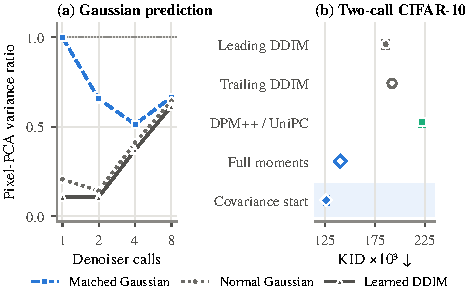
\includegraphics[width=\linewidth]{../figures/initialization_repair.pdf}
\caption{Correcting the initial covariance improves two-call generation.
(a) Fresh confirmation over five generated-sample panels; whiskers are
95\% intervals. (b) Gaussian predictions and learned DDIM in a common
teacher-fit pixel basis separate initialization from integration.}
\label{fig:cifar_initializer}
\end{figure}

\Cref{eq:gaussian} predicts the useful regime: standard-normal-to-matched
aggregate variance ratios are 0.216, 0.800, and 0.968 at two, four, and
eight calls. Learned trajectories correlate with the Gaussian prediction
at four/eight calls (Spearman 0.938/0.894). At these larger budgets,
full-moment initialization gives KID 0.0926/0.0378 versus DDIM's
0.0903/0.0363 (Supp.~Secs.~D--F), concentrating the benefit at the
smallest budget.

The repair improves real-data discrepancy and coverage. Concentration in
the largest teacher region falls from 97.30\% to 91.29\%, while the
fraction within the real-training 1--99\% frequency range rises from
0.72\% to 24.7\%. Evaluating the same outputs against CIFAR-10.1v6 lowers
KID from 0.19060 to 0.12832 (32.7\%) and raises coverage from 0.3221 to
0.4268. The paired KID difference is $-0.06228$
[$-0.06422,-0.06035$], with 95\% simultaneous coverage across four
contrasts (Supp.~Sec.~F.4). Supp.~Sec.~N.1 reports the remaining
teacher-relative deficit and precision change.

\subsection{Intervention location separates spread from useful coverage}
\label{sec:numerical}
At four calls, output covariance restoration raises pixel spread from
0.376 to 0.917, yet coverage falls from 0.478 to 0.332 and KID rises
from 0.0903 to 0.1024 (Fig.~\ref{fig:numerical_repair}). UniPC instead
reaches coverage 0.549 and KID 0.0694. At eight calls, output restoration
again raises KID (0.0363 to 0.0505), while UniPC reaches 0.0245
(Supp.~Sec.~F.2). The audit distinguishes restored spread from improved
real-data coverage.
\begin{figure}[t]
\centering
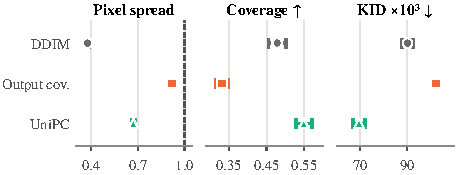
\includegraphics[width=\linewidth]{../figures/numerical_repair.pdf}
\caption{Restoring output spread can degrade useful coverage (four-call
CIFAR-10, five paired panels). Pixel spread is teacher-relative; coverage
and KID use real data.}
\label{fig:numerical_repair}
\end{figure}
The same discipline transfers to a second, independently pretrained
checkpoint (Fig.~\ref{fig:edm_solver_audit}). On the EDM model, Heun lowers
KID from 0.00876 to 0.00250 at 15 calls and from Euler's 0.00250 to
0.000413 at 35 calls, with coverage 0.501 for both solvers at 35 calls.
At 15 calls the audit also exposes a coverage trade-off that KID alone
hides, from 0.477 to 0.417. Small-budget behaviour and the frequency check
are in Supp.~Sec.~N.2.

\begin{figure}[t]
\centering
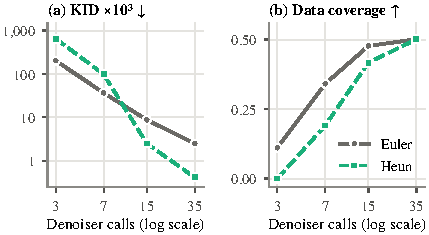
\includegraphics[width=\linewidth]{../figures/edm_solver_audit.pdf}
\caption{EDM solver choice changes with budget. Points are descriptive,
without model-seed uncertainty.}
\label{fig:edm_solver_audit}
\end{figure}

\subsection{Signed mass measurements enable calibrated semantic repair}
\label{sec:mnist}
Signed mass measurements reveal an overcorrection that a depletion test
cannot see, and ordinary continuation repairs it. They distinguish missing
probability from excess probability (Supp.~Sec.~H.2). Withholding digit~3
creates persistent real-data-relative depletion under DDIM25, DDIM50, and
DPM++25 in all three training seeds. At DPM++25, ordinary restoration
raises digit-3 mass from 0.00087 to 0.08747, toward the data target
0.0983; the adjusted paired increase is 0.08660 [0.07677,0.09643].
Coverage rises from 0.727 to 0.777, and the declared
five-percentage-point fidelity margins pass against the full-data control.
Doubling the restored digit's training weight overshoots to mass 0.1618. At equal updates, ordinary continuation reduces class-mass error by
58.7\% and digit-3 error by 89.1\% (Table~\ref{tab:repair-summary}).
The ordinary and targeted branches assign 9.08\% and 16.67\% of outcomes
to digit~3, against the real reference's 9.83\%. All four precision and
consensus fidelity constraints pass, and acceptance matches the full-data
control. Both error reductions also hold under DDIM25/DDIM50; digit-3
equivalence within $\pm0.03$ holds in all nine ordinary-continuation
seed--sampler probes. Diagnosis costs 48,000 images and 1.6 million
denoiser calls per checkpoint (Supp.~Sec.~H.2).
\begin{figure}[t]
\centering
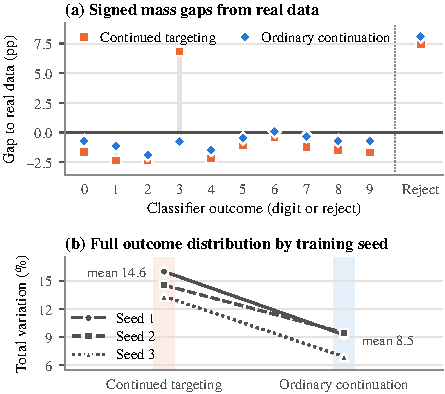
\includegraphics[width=\linewidth]{../figures/mnist_full_balance.pdf}
\caption{Ordinary continuation reduces imbalance across all classifier
outcomes, including rejection. (a) Mean signed gaps to real data.
(b) Total variation per training seed at 8,000 updates.}
\label{fig:mnist-full-balance}
\end{figure}
Across all eleven classifier outcomes, including rejection, total
variation falls from 0.1461 to 0.0854 (41.6\%), with descriptive paired
difference $-0.0608$ [$-0.0828,-0.0387$]
(Fig.~\ref{fig:mnist-full-balance}). Improvement holds in all three seeds.
On CIFAR-10 semantic regions, ordinary continuation improves DPM25 KID
from 0.01479 to 0.01010 and ten-region mass error from 0.0247 to 0.0148.
Both improve under all five samplers, fidelity constraints pass, and both
outperform event-ratio weighting under all three long-step probes.
Reference refinement and further controls appear in Supp.~Sec.~N.3.

\subsection{Crossed probes separate sampler deficits from persistent depletion}
\label{sec:crossed-probes}
Crossed probes distinguish deficits responsive to longer sampling from
depletion persisting across qualified samplers. All 12 short-sampler
cases from withheld training states retained digit-3 depletion under
three resolved probes and received sampler and training recommendations.
The other 18 received a sampler test; an occupancy-only rule would send
nine to retraining. On fresh samples, longer sampling improves
class-mass error, coverage, and acceptance in all 18. For persistent
cases, ordinary restoration with the resolved sampler raises digit-3
mass to 0.08567 versus 0.00067 under continued withholding at equal
updates. Cost and remaining contrasts appear in Supp.~Sec.~N.4.

\subsection{Conditioning and reference matching resolve diversity reversals}
\label{sec:t2i}
Exploratory comparisons show that pooling and teacher choice can reverse
the measured direction of diversity. DDIM4 has pooled DINO spread ratio
0.919 [0.910,0.928] but within-prompt ratio 1.306 [1.236,1.382]
(Fig.~\ref{fig:t2i_representations}). Within-prompt variation rises from
0.400 to 0.523 of reference pooled spread, while the between-prompt
component falls from 0.600 to 0.396, bringing the sum below one.
Sampling-latent and image-re-encoding ratios are 0.414 and 0.482; the
increased feature spread accompanies lower learned preference
(Supp.~Sec.~N.5).
\begin{figure}[t]
\centering
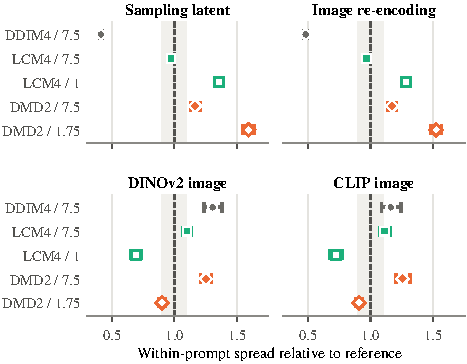
\includegraphics[width=\linewidth]{../figures/t2i_representation_reference.pdf}
\caption{Conditioning and reference matching change the measured direction
of within-prompt spread (descriptive intervals). Rows give sampler and teacher CFG; open markers
use the alternate teacher. The band marks $[0.9,1.1]$.}
\label{fig:t2i_representations}
\end{figure}
Matching the teacher changes the conclusion about a distilled model. DMD2's
DINO ratio moves from 1.251 [1.208,1.297] against CFG7.5 to
0.901 [0.873,0.929] against its matched CFG1.75 teacher; against that
teacher, latent spread increases to 1.592 and learned preference reaches
0.558 [0.545,0.571]. Sana Euler8 reduces latent spread to 0.763
[0.746,0.779] while DINO spread rises to 1.118 [1.083,1.157]. At eight
calls, Flow-DPM++ retains paired learned preference within tolerance,
0.479 [0.471,0.487]. CADS increases DINO spread to 1.965 [1.828,2.121] but
lowers preference to 0.354 [0.339,0.369].

\subsection{Validation makes the diagnostic resolution explicit}
\label{sec:supportcontrols}
Controlled deletions confirm that the audit resolves the deficits it is
designed to find, including ones that marginal and projected tests miss.
Removing one joint Gaussian component while retaining all marginal modes
is detected in 200/200 trials at 1,000 samples per set. NDB also detects
every joint removal, while both projected rules detect 0/200. Combined
removal, contraction, and translation produce all three labels in 200/200
trials. Rotation yields support departure in 198/200 trials with no
expansion. On cached image features, removing a 4.19\%-mass region is
detected in 0/200, 196/200, and 200/200 trials at 250, 1,000, and 4,000
samples per set (Supp.~Sec.~C).

Rare-region detection follows the sample-planning bound
(\cref{eq:planning}): for complete removal of a 1\%-mass region,
detection rises from 3.25\% at $n=2{,}000$ to 99.9\% at $n=5{,}000$
($M=10$, $\rho=0.5$, $\alpha_{\rm occ}=0.025$, eligibility 0.001;
2,000 trials per setting; Supp.~Fig.~1). At the true ratio 0.5 and
$n=5{,}000$, NDB flags change in 83.4\% of trials while the certificate
makes no below-threshold claims (Supp.~Sec.~C.5). This distinguishes a
detectable change from a certified loss of the declared magnitude. Across DINO PCA dimensions $\{16,32,64\}$ and $K\in\{5,10,20\}$
(525 regions in one exact family), four of five CIFAR-10 configurations
remain depleted in all nine settings; UniPC4 is depleted in seven.
All five remain contracted and pass support, confirming that the
principal findings persist across the tested representations and
partitions (Supp.~Secs.~C, N.6).

\subsection{What the audit establishes about choosing a sampler}
\label{sec:policy}
As a selector, the audit explains its choices while remaining close to
the strongest tested alternatives. Mean CIFAR KID is 0.0790 across two,
four, and eight calls, versus 0.1039 for leading DDIM and 0.0784 for
Vendi and teacher-feature Fr\'echet selection. The text-to-image policy
screens two fast samplers and uses a longer fallback when neither meets
the thresholds. Its independent outcomes pass fidelity and spread gates,
as do quality plus Vendi and fixed Sana DPM++8. It uses 14.06/14.28
denoising calls per image for Stable Diffusion/Sana, plus 528 diagnosis
calls per prompt and 38,400 reusable reference calls per family.
Thresholds, amortization, and matched-cost comparisons are reported in
Supp.~Secs.~J--L and~N.7.

Our fixed-reference audit turns generative diversity assessment into a framework for locating, quantifying, and repairing distributional gaps. By separating regional probability, conditional spread, and reference support, it makes changes in a generator’s output distribution interpretable and actionable. Finite-sample certificates establish the magnitude of regional mass changes, explicit sample requirements define the audit’s resolution, and controlled interventions test whether a diagnosis leads to improvement on independent outcomes. The experiments demonstrate this connection at matched computational budgets. Covariance initialization reduces two-call CIFAR-10 KID by 32.0\% and improves real-data coverage without additional denoiser calls, with gains retained against CIFAR-10.1. Ordinary continuation reduces MNIST class-mass error by 58.7\% at equal training updates and improves total variation across all classifier outcomes, including rejection. Gaussian analysis separates initialization from integration error, while crossed probes distinguish sampler-sensitive deficits from persistent depletion. Across four text-to-image families, the audit reveals diversity reversals caused by pooling, representation, and teacher choice. Together, these results establish a practical link between statistically grounded distributional diagnosis and targeted generator improvement, giving practitioners a concrete basis for deciding what to change.
\label{audit:lastbodypage}
\clearpage
\section*{LLM Usage Statement}
OpenAI ChatGPT assisted with manuscript editing, clarity, and figure planning.
OpenAI Codex assisted with manuscript and caption revisions, the illustrative
toy example, notation and numerical checks, LaTeX preparation, internal
critical review, plotting, table generation, and preparation of an earlier
pipeline diagram. Codex also assisted with the abstract, introduction, related
work, methods, and results synthesis, including a table assembled from existing
measurements, and provided internal draft assessments. Codex also generated the
classifier-event balance analysis and computed its secondary paired summary
from saved outcomes. An earlier project record contains an AI-generated
manuscript review whose tool is unrecorded. BioRender assisted with diagram
formatting and icons in an earlier version of Figure~1. Anthropic Claude
assisted with the current revision: redrawing all figures in the main paper,
recovering plotted values from earlier figure files and checking them against
the reported numbers, restructuring the text, and verifying that every reported
number was retained. The authors are responsible for the scientific claims.

{\small
\bibliographystyle{ieeenat_fullname}
\bibliography{references}}
\end{document}
